\documentclass[11pt]{article} 
\usepackage[utf8]{inputenc}
\usepackage{geometry}
\usepackage{sgame}
\geometry{
    letterpaper,
    total={6.5in,9in},
    left=1in,
    top=1in,
}
 \usepackage{graphicx}
 \usepackage{titling}
 \usepackage{url}

 \usepackage{amsmath}
\usepackage{tikz}
\usepackage{hanging}
\usepackage{changepage}


\title{Sleep, Sociology, and Evolutionary Dynamics on Graphs}
\author{Joshua Lau}
\date{Fall 2024}
 
 \usepackage{fancyhdr}
\fancypagestyle{plain}{%  the preset of fancyhdr 
    \fancyhf{} % clear all header and footer fields
    % \fancyfoot[L]{\thedate}
    \fancyhead[L]{COS597C Final Paper}
    \fancyhead[R]{\theauthor}
}
\makeatletter
\def\@maketitle{%
  \newpage
  \null
  \vskip 1em%
  \begin{center}%
  \let \footnote \thanks
    {\LARGE \@title \par}%
    \vskip 1em%
    %{\large \@date}%
  \end{center}%
  \par
  \vskip 1em}
\makeatother

\usepackage{lipsum}  
\usepackage{mathptmx}
\begin{document}

\maketitle

\noindent\begin{tabular}{@{}ll}
    \textbf{\theauthor}, Department of Electrical \& Computer Engineering, Princeton University\\
    \textbf{Bernard Chazelle}, Department of Computer Science, Princeton University
\end{tabular}

\section*{Abstract}
\textit{Analyzing evolutionary dynamics presents a significant  challenge due to its high-dimensional and stochastic nature. By studying simplified game-theoretic models of evolution, we can extract the principles that govern optimal strategy selection. This paper synthesizes key findings from the literature on game-theoretic evolutionary dynamics, especially those on graphs, examining both their theoretical foundations and broader implications for understanding social behavior and philosophical questions. We extend previous work by introducing sleep as a novel parameter in graph-theoretic evolutionary models. Our analysis provides potential insights into how sleep could evolve as an optimal strategy. We also suggest future directions that bridge the gap between empirical research and theoretical models.}

\section{Introduction}
There are two primary methods with which evolutionary dynamics can be studied. First, researchers in experimental sciences and social sciences collect empirical data through experiments, field studies, and observations, then develop statistical models to explain these findings. This \textit{data-first} approach prioritizes real-world observations and uses mathematics primarily as a tool to describe and analyze collected information. The second approach starts with mathematical models based on simple observations from nature, then explores their theoretical implications. Rather than being driven by specific datasets, this \textit{model-first} strategy aims to uncover fundamental principles that might govern evolutionary systems. While both approaches offer valuable insights, this paper focuses on the model-first perspective, examining how abstract graph-theoretic frameworks can illuminate evolutionary dynamics.

A data structure that is well suited to model evolutionary dynamics is the graph since it can model arbitrary types of nodes, relationships between those nodes, and can be modified to evolve over time. When considering these evolving graphs, we can view them from a game-theoretic perspective, giving nodes different strategies and determining which strategies are favorable under a set of conditions. In this paper, we describe the foundational works of game theory on graphs with regard to evolutionary dynamics, the implications of these works, and discuss an original case about sleep. 


\section{Previous Work}
Our overview of evolutionary dynamics on graphs will follow the explanation found in Ohtsuki et al. (2006) and their corresponding supplementary materials. Note that this section is not original -- it is a restatement of their work with commentary that is intended to make some aspects clearer. We will then describe related work in theoretical evolutionary dynamics. Finally, we conclude this section by mentioning some original sociological and philosophical insights. 

\subsection{Overview}
Imagine that we have some fixed amount of nodes $N$. There are 2 different strategies a node can have. It can be a \textit{collaborator}, meaning that it pays a cost of $c$ for each neighbor it has, while its neighbors receive a benefit of $b$. It can also be a \textit{defector}, meaning that it pays no cost and its neighbors receive no benefits from it. Consider a node that is connected to $k$ neighbors, with $i$ of those neighbors being collaborators. If the node is a collaborator, its payoff will be $bi - ck$, while if the node is a defector, it will simply receive a payoff of $bi$. At first glance, it may seem as if defectors will always be favored in any update mechanism since $bi \geq bi - ck$. However, as Ohtsuki et al. (2006) reveal, this is not the case in all situations.

First, we define the fixation probability as the probability that if all nodes have one strategy, and a single node takes on a different strategy, that eventually all nodes will have that different strategy. In other words, if $N-1$ nodes have strategy $A$ and $1$ node has strategy $B$, the fixation probability is the probability that all $N$ nodes will eventually have strategy $B$. It is clear that if the fixation probability is greater than $1 / N$, then strategy $B$ is favored. This is because if the fixation probability is $ 1/ N$, it would imply that strategy $B$ is equally as strong as strategy $A$. Let strategy $A$ be defectors and let strategy $B$ be collaborators. 

We consider a few different update mechanisms. First, in death-birth updating, a node is picked uniformly at random to be killed. Then, that node is replaced by a node with the strategy determined probabilistically by the fitness of its neighbors. Intuitively, death-birth updating can be favored in some situations. Figure 1 demonstrates how when considering what strategy to replace the empty node, the fitness of the collaborator is $b - c$ while that of the defector is $0$. So long as $b > c$, the collaborator would have more fitness. This assumes a few things: this is a simple ring graph and the collaborator at the junction has only a collaborator neighbor. Fortunately, as we will see, this generalizes beyond ring graphs and collaborators are more likely to have collaborator neighbors. 

\begin{figure}[htbp]
    \centering    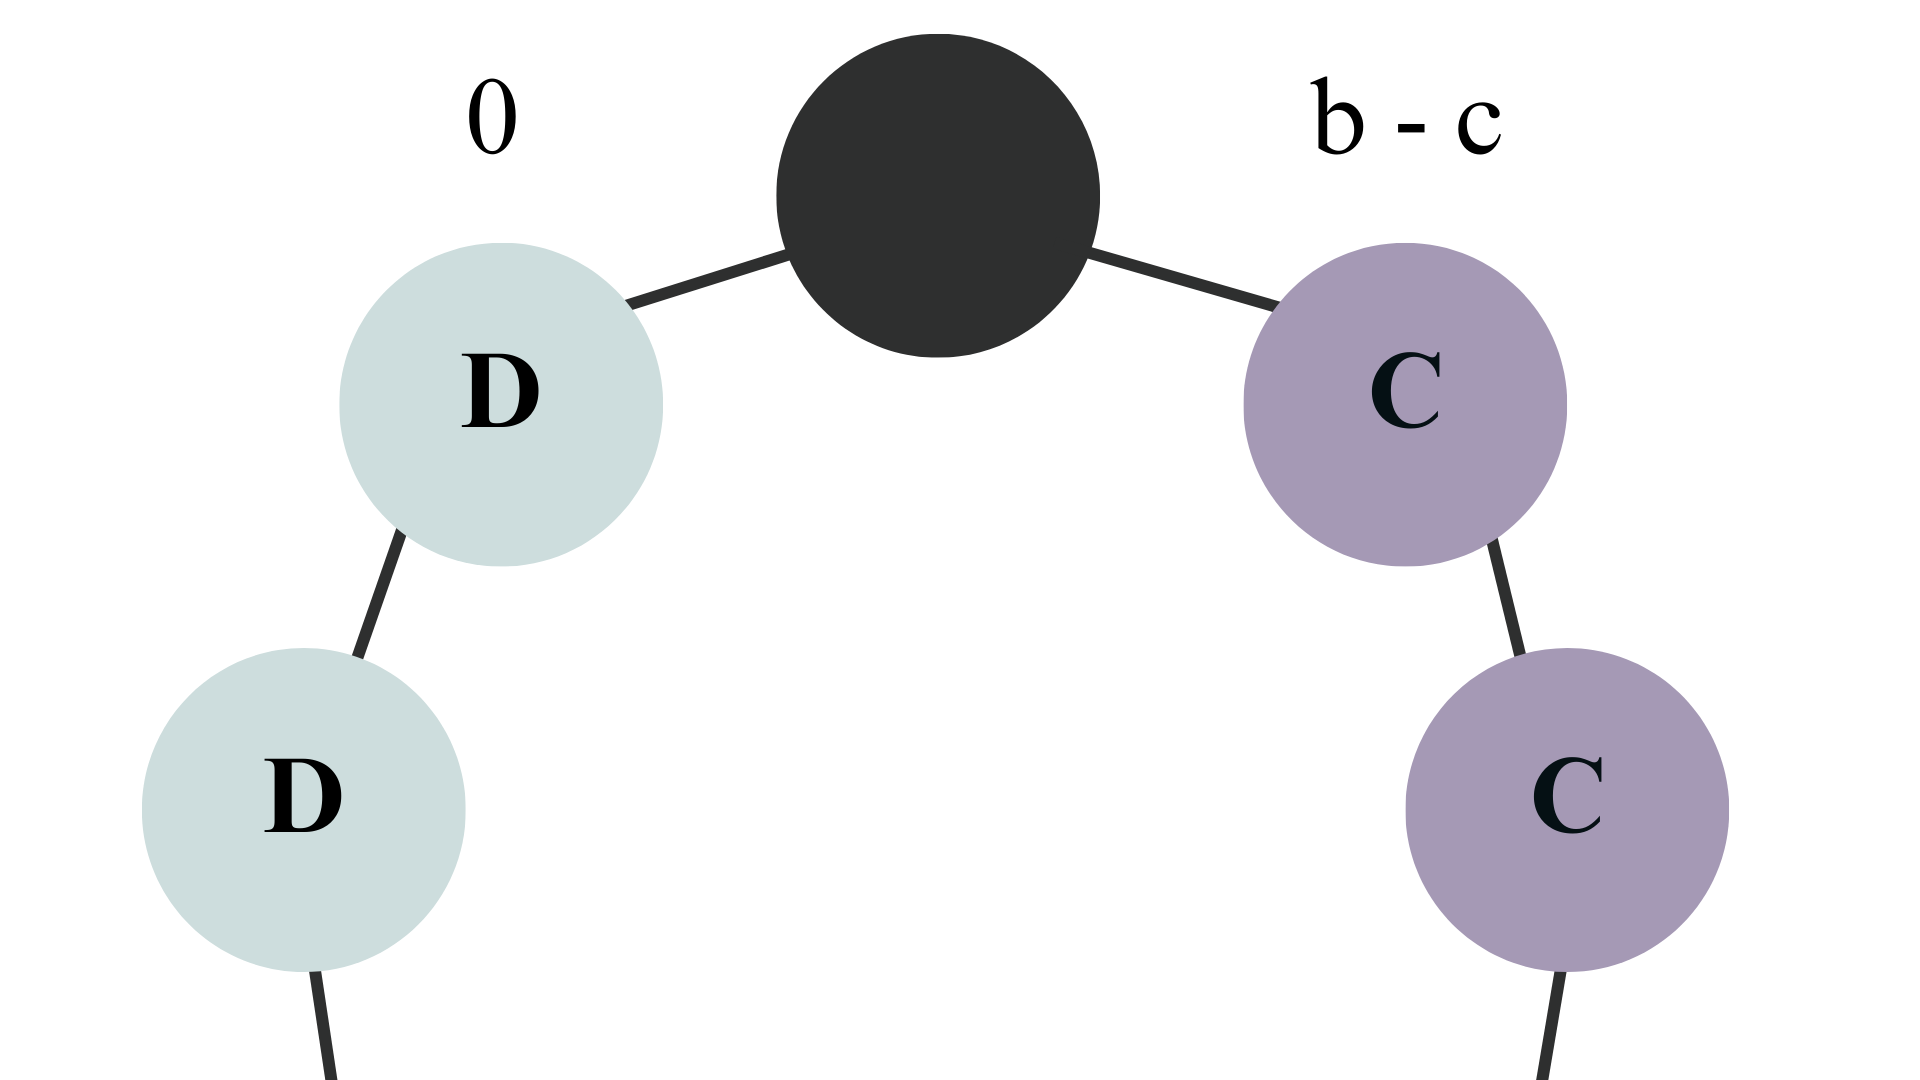
\includegraphics[width=0.5\textwidth]{figures/death-birth.png}
    \caption{A simple ring graph that demonstrates that it is possible for collaborators to be favored with the death-birth update mechanism.}
    \label{fig:death-birth}
\end{figure}

Before discussing an analytical solution to when collaborators are favored, we first introduce some notation. $p_X$ is the frequency of some strategy $X$ in a population. $p_{XY}$ is the frequency of $XY$ pairs. $q_{X|Y}$ denotes the conditional probability of finding an $X$ player given that the adjacent node is occupied by a $Y$-player. This last probability is perhaps the most confusing, but intuitively it means that if we are looking at a $Y$ player, what is the probability that a randomly selected neighbor is an $X$ player. This is an intuitively useful probability because the composition of neighbors directly determines the payoff (and thus fitness) of a node. 

We now consider a general payoff matrix for any 2 strategies. We solve for when a strategy in an arbitrary pair of strategies is favored, and then map this general solution onto our specific solution. This helps with cleanliness of notation and also generalizes the solution to multiple strategies:

\begin{equation}
    \begin{bmatrix}
        a & b\\
        c & d
    \end{bmatrix}
\end{equation}

We want to have the notion of intensity of selection. That is, we want to have some parameter where at its maximum, fitness is directly proportional to payoff, while at its minimum, all nodes have equal fitness regardless of payoff. This is to help model real-world evolutionary scenarios where there is often noise. Let $w\in[0,1]$ represent this intensity of selection, with $w = 1$ meaning fitness equals payoff, and $w=0$ meaning payoff is irrelevant. 

First, let's consider the case that a $B$ player was killed. We want to determine the probability $P(A)$ that an $A$ player replaces the vacancy, and also the corresponding probabilities that $p_A$ and $p_{AA}$ increase. We can define the fitness of the $A$ and $B$ neighbors as:

\begin{equation}
    f_A = (1 - w)  + w[(k-1)q_{A|A}\cdot a + ((k-1)q_{B|A}+1)\cdot b]
\end{equation}

\begin{equation}
    f_B = (1 - w)  + w[(k-1)q_{A|B}\cdot c + ((k-1)q_{B|B}+1)\cdot d]
\end{equation}

We utilize the $q$ values in order to determine the expected neighbor composition for each of the neighbors of the vacant node, and then multiply those by the payout of the interaction. We use $k - 1$ instead of just $k$ because $k$ is the average number of neighbors, but 1 neighbor is vacant. From this, we can define the probability that a vacant node is replaced by strategy $A$ as:

\begin{equation}
    P(A) = \frac{k_A f_A}{k_Af_A + k_Bf_b}
\end{equation}

$P(B)$ can be derived similarly. We can check the boundary conditions of this function by noting that if $f_B = 0$, then $P(A) = 1$ and if $f_A = 0$, then $P(A) = 0$. We then calculate the corresponding probabilities:

\begin{equation}
    P\left(\Delta p_A = \frac{1}{N}\right) = p_B \sum{k_A + k_B = k}\frac{k!}{k_A!k_B!}q_{A|B}^{k_A}q_{B|B}^{k_B}P(A)
\end{equation}

\begin{equation}
    P\left(\Delta p_{AA} = \frac{2k_A}{kN}\right) = p_B \frac{k!}{k_A!k_B!}q_{A|B}^{k_A}q_{B|B}^{k_B}P(A)
\end{equation}

These follow directly from the probability that a $B$ node was killed, the composition of the neighbors, and the probability that the vacant node is replaced by a node of strategy $A$. 

Now, we want to consider the case that an $A$ player is killed. In this scenario, it is impossible for $p_A$ or $p_{AA}$ to rise since the best case scenario is that they remain the same. Using analogous logic to when a $B$ player was killed, we can determine first that the fitness of the strategies is:

\begin{equation}
    g_A = (1 - w) + w\left[((k-1)q_{A|A} + 1) \cdot a + (k-1)q_{B|A}\cdot b \right]
\end{equation}

\begin{equation}
    g_B = (1 - w) + w\left[((k-1)q_{A|B} + 1) + (k-1)q_{B|B}\cdot d\right]
\end{equation}

Then, we note that the probability that a $B$ player fills the space is:

\begin{equation}
    P(B) = \frac{k_Bg_B}{k_Ag_A + k_B g_B}
\end{equation}

Finally, we calculate the desired analogous probabilities:

\begin{equation}
    P\left(\Delta p_A = -\frac{1}{N}\right) = p_A \sum_{k_A + k_B = k} \frac{k!}{k_A!k_B!}q_{A|A}^{k_A}q_{B|A}^{k_B}P(B)
\end{equation}

\begin{equation}
    P\left(\Delta p_{AA} = -\frac{2k_A}{kN}\right) = p_A \frac{k!}{k_A!k_B!}q_{A|A}^{k_A}q_{B|A}^{k_B}P(B)
\end{equation}

To reiterate we have now determined equations for the probabilities that $p_A$ and $P_{AA}$ will increase or decrease by 1 unit. We can now use these probabilities to solve for the dynamics of the system. However, these dynamics are quite complicated, so we can use diffusion approximation to approximate the dynamics into a solvable state. Diffusion approximation is a technique where we model the dynamics based on diffusion processes -- instead of examining each node individually, we analyze the average of the system as a whole and notice, in this case, how the strategies spread over time. 

\begin{equation}
    \dot{p_A} = \frac{1}{N}\cdot P\left(\Delta p_A = \frac{1}{N}\right) - \frac{1}{N} \cdot P\left(\Delta p_A = -\frac{1}{N}\right)
\end{equation}

\begin{equation}
    \dot{p_{AA}} = \sum_{k_A = 0}^k \frac{2k_A}{kN} \cdot P\left(\Delta p_A = \frac{2k_A}{kN}\right) - \sum_{k_A = 0}^k \frac{2k_A}{kN} \cdot P\left(\Delta p_A = -\frac{2k_A}{kN}\right)
\end{equation}

We can expand these expressions to eventually reach the conclusion that an $A$ node has on average one more $A$ neighbors compared to a $B$ node. This supports our initial remarks. From the expanded equations, we can also explicitly calculate the fixation probabilities. The only additional assumption that must be made is that $w$ is very small, meaning that there is weak selection. It makes intuitive sense that weak selection would be necessary for collaboration to be reasonably favored. Early on, when there are few (or even only 1) collaborator nodes, then it would be very difficult for collaborators to spread with strong selection. For analytic simplicity, a large $N$ is also assumed. See Ohtsuki et al. (2006) for a full explanation on how the expanded equations and dynamics are derived (in this paper, we are focusing on more of a conceptual overview). 

Finally, we transform the general payoff matrix into the specific collaborator-defector matrix. 

\begin{equation}
    \begin{bmatrix}
        a & b \\
        c & d 
    \end{bmatrix}
    \rightarrow
    \begin{bmatrix}
        b - c & -c\\
        b & 0
    \end{bmatrix}
\end{equation}

By substituting these values into our expanded equations, it can be proved that fixation probability of collaboration is greater than $1 / N$ if and only if $ b / c > k$ given that there is weak selection and a large population size. 

For the following update mechanisms, we will discuss only the conceptual overview and results. The mathematical explanation of the death-birth updating was to demonstrate that there can be analytical solutions to these games in some cases. However, even our explanation revealed some of the limitations of analytical solutions. 

A mechanism with a similar result to death-birth updating is imitation updating. In this mechanism there is no birth or death. Every round, a node is picked uniformly at random to imitate the strategy of one of its neighbors probabilistically dependent on the fitness of the neighbors. This mechanism is seemingly very similar to death-birth updating, except that the node being considered is counted as a neighbor to its neighbors, as opposed to death-birth where the node considered is a vacant spot that has no influence on its neighbors. The primary insight of death-birth updating that allows collaboration to sometimes prosper is that collaborative nodes have, on average, 1 more collaborative neighbor. While this is still true, when considering a collaborative node, both defectors and collaborators will have 1 extra collaborative neighbor, and when considering a defector node, the collaborators will pay 1 extra cost. 

Intuitively, this should make it so that collaborators are slightly less favored with imitation updating. Indeed, the authors show that collaboration is favored if $b / c > k + 2$. When $k$ is relatively small, imitation updating places a large penalty on collaboration, but when $k$ is relatively large, this nearly reduces to the death-birth case. This makes sense because we are adding a constant 1 extra collaborator or defector to the fitness of each node, which is a relatively small change when $k$ is large. Figure 2 visualizes this point on a ring graph. 

\begin{figure}[htbp]
    \centering    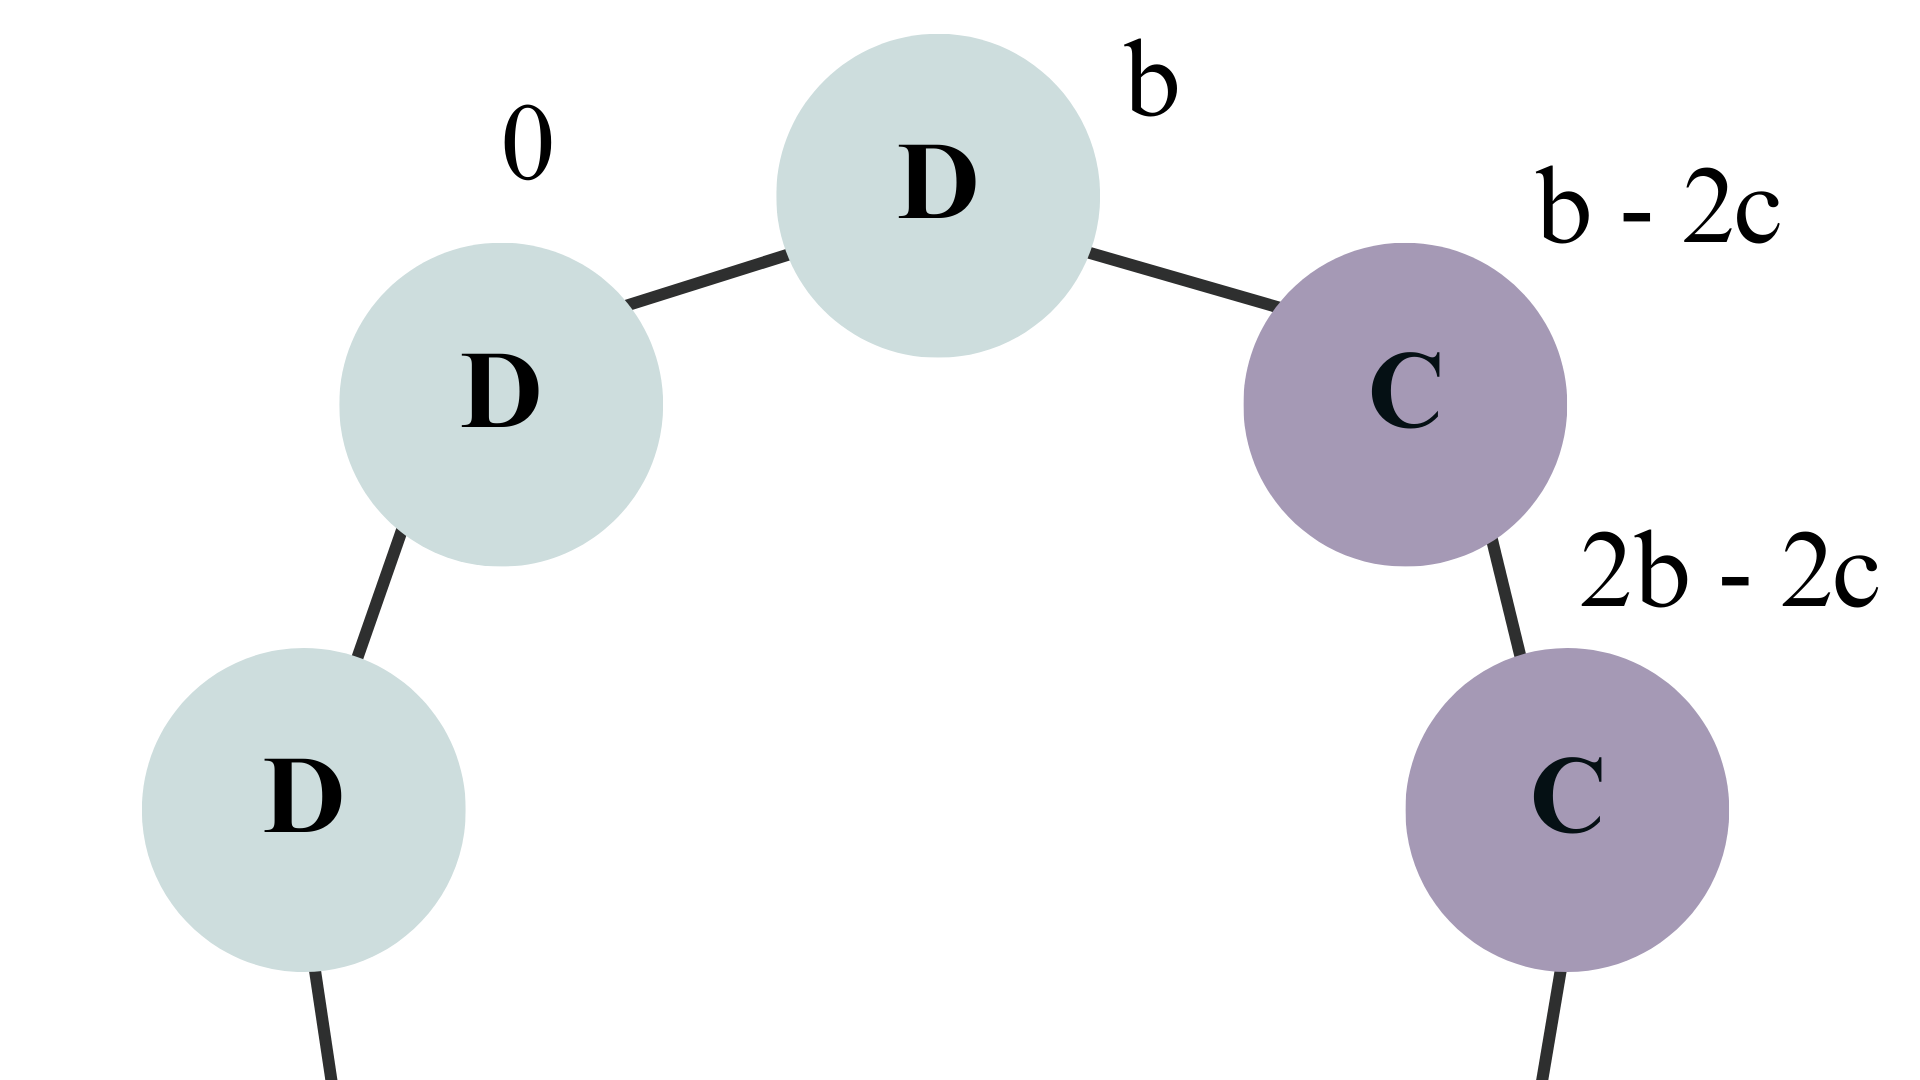
\includegraphics[width=0.5\textwidth]{figures/other-mech.png}
    \caption{With imitation updating, collaborators are slightly less favored compared to death-birth updating because there are more strict conditions on $b$ and $c$ that must hold for collaborators to have higher fitness (in this case $b > 2c$). With birth-death updating, it is impossible for collaborators to be favored because at the junctions, defectors will always have higher fitness. }
    \label{fig:other-mech}
\end{figure}


Some update mechanisms, however, never favor collaboration. In the birth-death update mechanism, we first select a node probabilistically according to fitness. Then, one of its neighbors is randomly replaced with a node that has the same strategy as the selected node. There is only a subtle difference with this mechanism compared to the other two. That is, the node that is selected is not picked at random, but rather based on fitness. In death-birth, the node that is eliminated is picked at random, and in imitation, the node that does the imitation update is also picked at random. 

This small change makes it impossible for collaboration to be favored. Conceptually, this is because defectors generally have higher fitness than collaborators. To make this model clear, consider the ring graph in figure 2. The only nodes that have any impact when selected are those at the junction between a collaborator and defector, otherwise, it is guaranteed that the state of the system will not change. At the junction, the defector will certainly have a higher fitness than the collaborator because the defector has fitness $b$ while the collaborator has fitness $b - c$. Therefore, it is more likely that the defector will be selected, so it is more likely that defectors will become the only node type regardless of $b$ or $c$. This $k = 2$ case can be generalized to larger $k$ analytically or numerically, but the same principles hold. 

To verify the game-theoretic solutions, computer simulations can be used to analyze the fixation probabilities through dynamic programming. While experimentally finding the probabilities through experimentation is more straightforward than solving for them analytically, the algorithms to run the simulations can be quite slow and run in exponential time. That said, for these types of complex problems, simulations are often one of the best ways to find results. Create a simulation that returns true if all nodes become collaborators, and false if they become all defectors. Note that we will always reach one of these cases -- there are no conditions where collaborators and defectors can coexist in perpetuity. Ohtsuki et al. (2006) simulated all three of the aforementioned update strategies and confirmed their theoretical rules.

\subsection{Other Works}

Prior to Ohtsuki et al. (2006), Lieberman et al. (2005) laid the foundations for evolutionary dynamics on graphs. Prior to this work, evolutionary dynamics was more constrained in the population structure. By allowing evolutionary dynamics to play out on graphs, there can be arbitrarily complex population structures with heterogenous populations. The work describes a weighted, directed graph in which edges represent the fitness at which nodes replace the other node with an offspring in the event that the other node is killed off. They also describe how previously studied structures of evolutionary dynamics are special cases of the graph model, demonstrating the generality and applicability of the graph model. 

Ohtsuki et al. (2015) followed up on their research on cooperative strategies in evolutionary dynamics by examining how reputation effects cooperation. In the 2006 work, it was assumed that collaborator nodes give the benefit and take the cost for each of its neighbors. In reality, individuals are much more likely to help other individuals that have a good reputation of reciprocity -- a mechanism termed indirect reciprocity. Not only are cooperative versus defective strategies explored, but also honest and hypocritical behaviors. Interactions are probabilistically determined to be either public or private, where public interactions are seen by all nodes while private interactions are only seen with some probability. Through dynamic programming, the authors found that always defecting is evolutionary stable, while the other conditions rely on the cost, benefit, probabilities of public versus private interaction, and how much nodes judge other nodes for having a low reputation score.  

Allen et. al (2017) further generalized the graph model by allowing nodes to have different numbers of neighbors. While this was briefly explored through simulations in Ohtsuki et al. (2006) with random graphs and scale-free networks, this work expands on that notion by exploring approximation methods for the NP-complete problem of deciding which strategies are favorable on an arbitrary graph. By calculating the coalescence times of random walks, they can do this analysis in reasonable time. In other words, since coalescence time is the expected meeting time of two random walks started at different vertices, this can be utilizes to analyze ancestral lineages. Ultimately, the authors determine that graphs with strong pairwise ties most encourage cooperation under weak selection. That is, 

Recently, Fujimoto \& Ohtsuki (2023) examined indirect reciprocity when individuals can individually decide their assessment strategy. In Ohtsuki et al.'s 2015 work, it was assumed that all nodes have the same assessment strategy; examples include Stern Judging (SJ), where cooperating with a bad node is judged as bad, and defection towards a bad node is judged as good, and Simple Standing (SS) where any action towards a bad node is good. In previous analyses where there is a global assessment strategy, both SJ and SS proved to allow stable cooperation even under noisy conditions. However, with private assessment, SJ is no longer ensures the stability of cooperation because there is too much error accumulation. The authors also point out that this makes intuitive sense -- SS favors cooperation towards bad nodes while SJ does not, sociologically indicating that errors in reputation can be more easily corrected through an SS-like strategy. 

\subsection{Sociological and Philosophical Implications}
The insights on evolutionary dynamics on random graphs can spur a myriad of philosophical implications about life and nature. The idea of collaborator versus defector could be taken in a biological sense, where fitness is literally the fitness of living. From a sociological perspective, these strategies could map towards aspects of behavior like kindness and philanthropy versus selfishness. From a geopolitical perspective, there could be insights about international alliances and foreign aid. In this section, we explore a few of these implications in depth. 

Of course, these analyses are meant to be taken with a grain of salt. The graph-theoretic games are absolutely not sufficient to capture the true, complex, noisy dynamics of biological and social evolutionary interactions. However, it is quite interesting to consider what implications can be formed by theoretical results in order to critically examine the relevance of the results, to guide future research, and to ground theory in reality. 

\begin{figure}[htbp]
    \centering    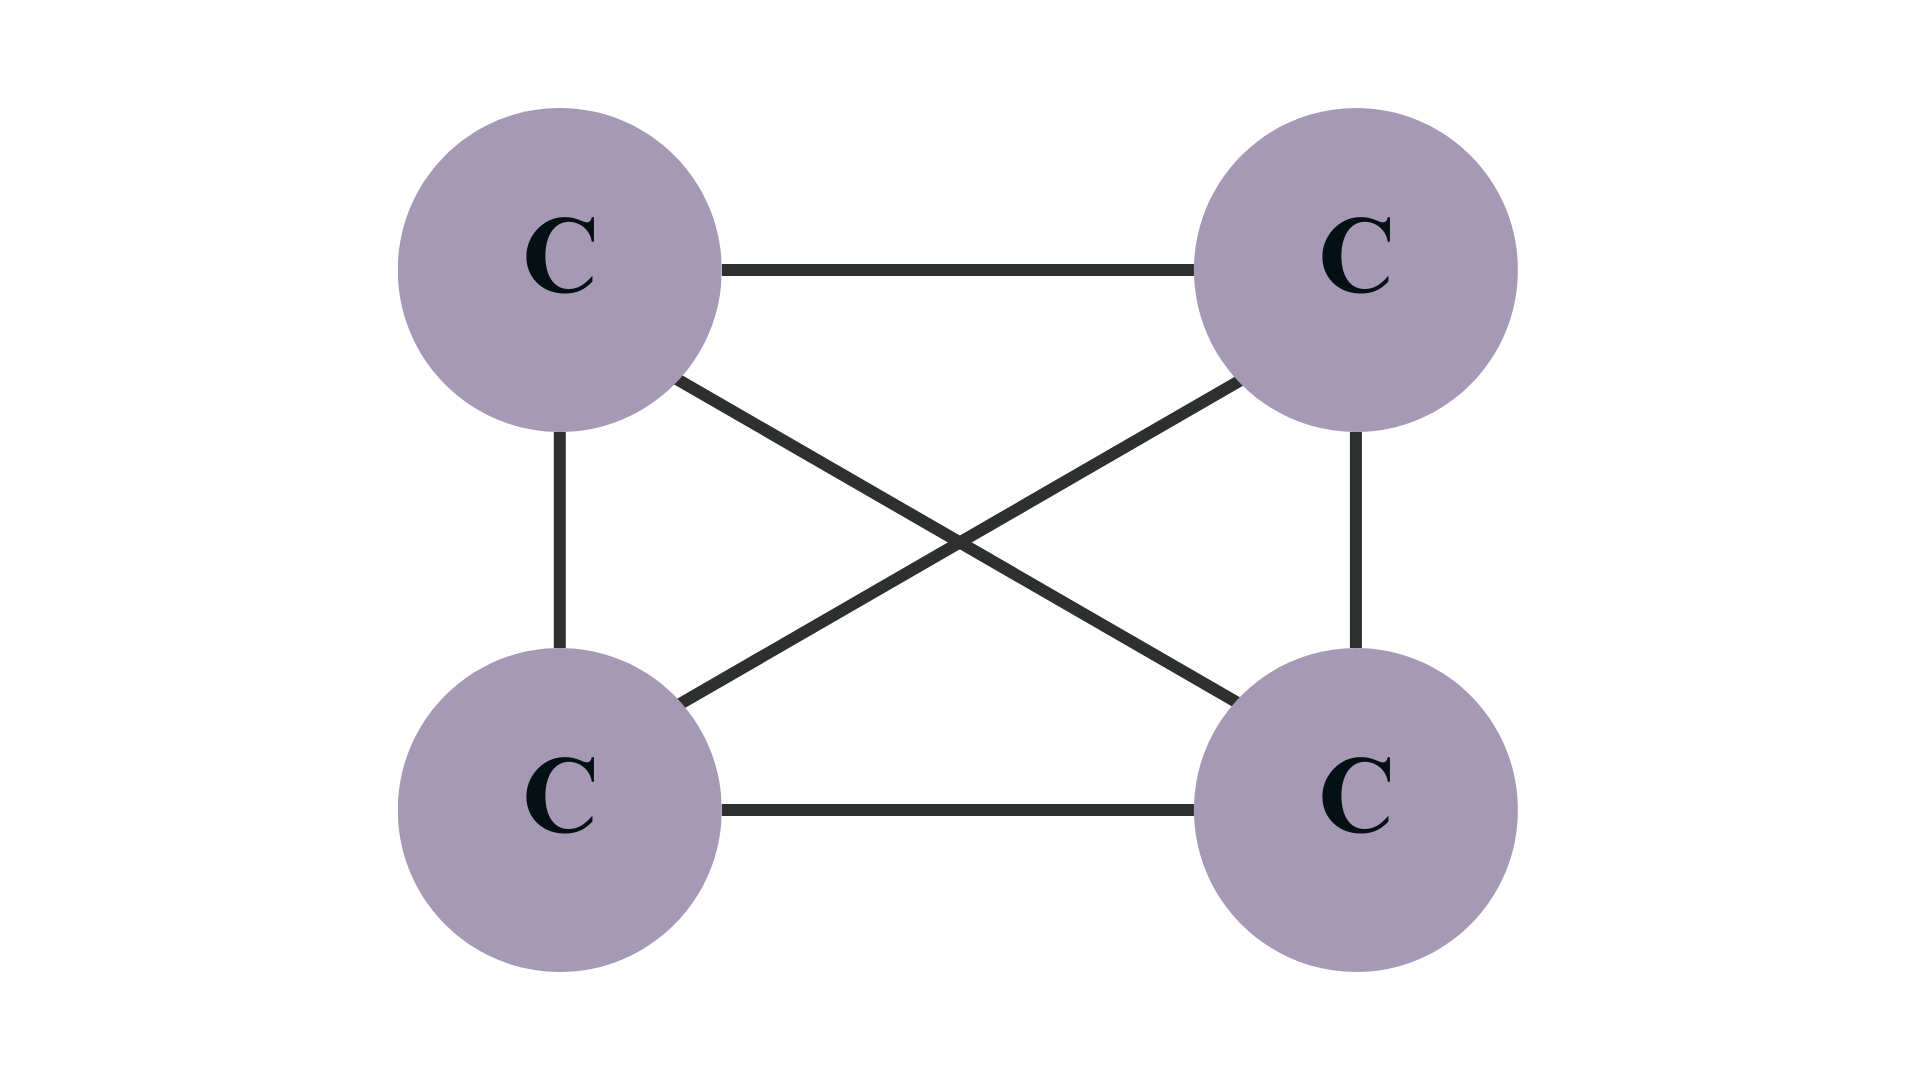
\includegraphics[width=0.5\textwidth]{figures/friends.png}
    \caption{A highly-connected graph with $k = 3$, simulating a group of close friends or communists.}
    \label{fig:friends}
\end{figure}

First, consider why you should give gifts to your family and friends this Christmas. Let's assume that the benefit of receiving a gift $b$ is larger than the cost of thinking of and buying a gift for someone $c$ (by benefit and cost we do not mean the literal monetary cost; we also factor in holistic factors like happiness). Imagine that you have 3 friends and that all of you are connected in a mutual friend group as shown in Figure 3. Therefore, $k = 3$. Since (hopefully) none of you die this Christmas season, we will consider the case of imitation updating, making $ b / c > k + 2 = 5$ be a requirement for collaboration to be favored. By this logic, the benefit of receiving a gift needs to be 5 times the value of purchasing a gift. We can make a few interesting observations based on this. $b/c$ needs to be relatively large even with such a small friend group since we are using imitation updating. If you had more friends, this ratio would be even larger! Now, you can attempt to buy really good gifts, or be nice to your friends to increase their positivity (and thus their perception of the gifts), or you could look for great deals to save on cost. Also, you better not add more friends to your friend group, otherwise it will become increasingly difficult to make collaborative gift-giving the dominant strategy. However, with a ratio like $b/c > 5$, it seems quite likely that collaboration will not be favored in many instances. 

Note that even if collaboration is not favored, if no one spontaneously changes from collaborating to defecting, then everyone will collaborate forever. However, if you think too much about this and decide to defect and give no gifts this Christmas in order to receive your greedy best-case payout this year, then you open the door to everyone eventually defecting (with probability higher than $1/4$ since defection is favored). Since we are assuming that $b > c$, everyone will be better off if collaboration is the dominant strategy since everyone will receive a positive payout (compared to if everyone defects where everyone gets 0 payout). Therefore, in the long run, your Christmas blunder harms everyone, including yourself. If everyone thinks the same way as you, the collapse of Christmas collaboration is all but inevitable. Of course, the model also implies that if no one gives gifts and collaboration is not favored, it may be futile to try this Christmas (or any Christmas). 

Another fun example: imagine a group of $N$ communists that all collaborate with each other. Let's assume that collaboration is favored under imitation updating ($b/c > N +1$). Every year, $n$ children are born and $m$ individuals die. Assume that children are naturally greedy and are born defectors. Also assume that $m, n \ll N$ Formally, every few rounds, remove $m$ nodes at random and add $n$ defectors (the graph remains fully connected). If $n \leq m$, then collaboration will continue to be favored in perpetuity (or at least until there are no nodes remaining). This does not preclude the situation where the graph turns to all defectors (since there is a nonzero probability of this happening at every child birth scenario, it is inevitable), but defection will never have a fixation probability higher than $1 / N$. On the other hand, if $n > m$, then the $b / c > N + 1$ initial condition that collaboration is favored will eventually not hold since $N$ increases and $b / c$ is a constant. These results suggest that communists should keep their fertility rates low so that their society does not collapse. 

On the other hand, some less logical claims can be made based solely on these results. For example, consider a pack of wolves in a forest. There is a fixed number of resources available in the forest, so there will always be $N$ wolves. Initially, the wolves do not work together: they are all defectors. Additionally, the most fit wolves are the ones that are able to have their offsprings replace a wolf when one dies. Assume that $b / c > k$. If we interpret this based on death-birth updating, then collaboration is favored, so if a wolf suddenly becomes a collaborator, then this strategy has fixation probability greater than $1/N$. On the other hand, if we interpret this based on birth-death updating, that is, a new wolf is born and a random one is then killed off, then collaboration will never be favored. Since, in reality, $N$ is not completely constant, it is likely that both of these mechanisms would be occurring. However, strictly based on the model, we get wildly different results depending on how we interpret the reproduction mechanisms of the wolves. 

A limitation of this work is that all 3 updating mechanisms assume that $N$ is fixed. In nature, this is often not true as population sizes change over time. The mechanisms are also not considered at play at the same time, which is most likely true for many biological and sociological situations. Furthermore, as demonstrated in the wolf-example, since there is only a subtle difference between birth-death and death-birth updating, but very different interpretations based on what strategy is considered "favorable", it brings into question if the definition of "favorable" based on fixation probability is the correct one to consider. 

\section{Sleep Dynamics}
We now use the principles of the previous work to briefly consider an novel case -- namely, when is the strategy of sleeping favored? According to some researchers, almost every single animal sleeps (Walker 2017). This is despite the fact that sleep seems counterintuitive; it is a state of defenselessness and prevents the animal from doing anything during that time. Imagine a human that did not have to sleep but still had the same level of energy as if they did -- they would have a massive advantage in almost all situations. Therefore, there must be some neurobiological explanation for why sleep is so prevalent. 

In this analysis, we simplify the notion of sleep. Consider a graph with $N$ nodes where each node has $k$ neighbors. We assume that all nodes are collaborators, that they give a benefit $b$ to their neighbors while taking on a cost $c$. For simplicity, since all nodes are collaborators and we are assuming that $b > c$ (otherwise collaboration would never make sense), we can reduce this to a single positive value $b$. Some nodes have strategy $A$ (stands for "awake") where they are the normal collaborators mentioned in the previous section. Other nodes can have strategy $S$ (stands for "sleep") where they have some multiplier $\lambda$ to their benefits given and received, but also have a $\alpha$ multiplier for their probability of death in the death-birth updating mechanism. We want to determine in what situations (if any) is the sleep strategy favorable (fixation probability $>1/N$). 

\begin{figure}[htbp]
    \centering    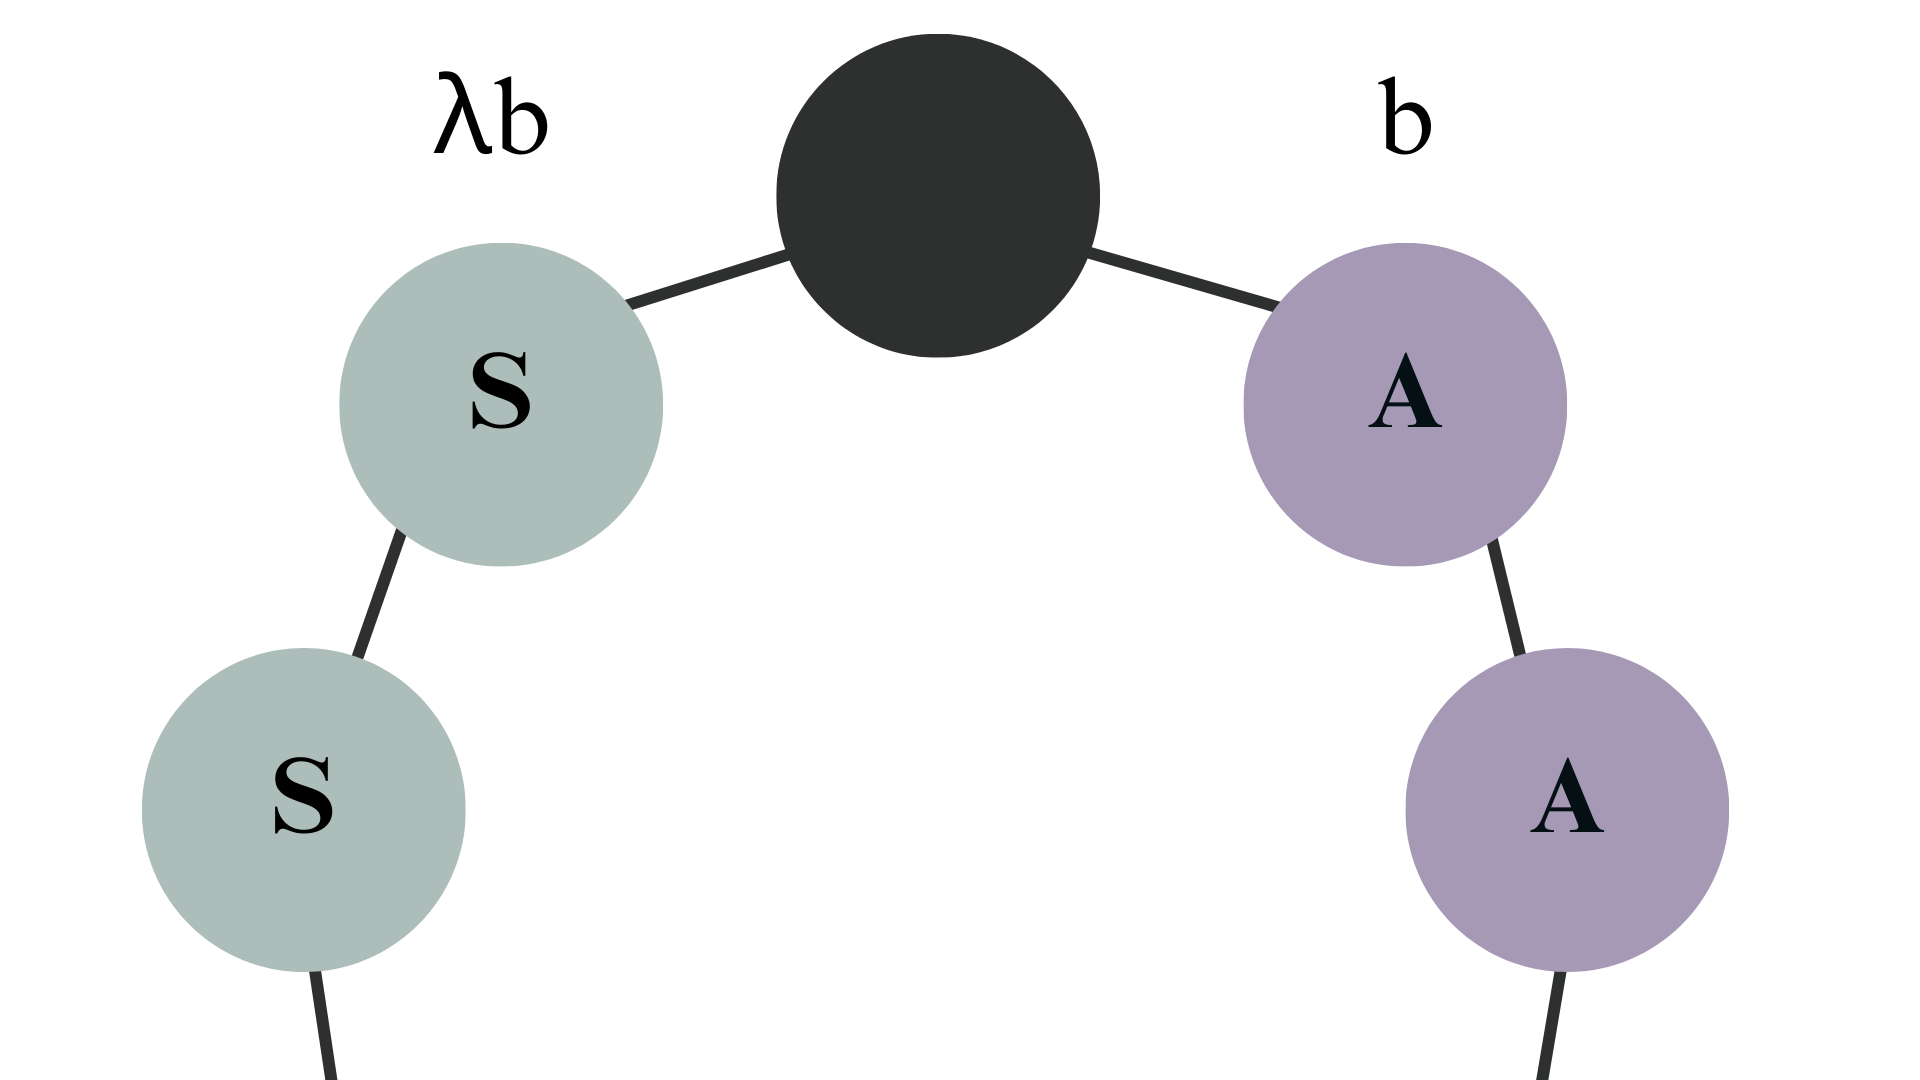
\includegraphics[width=0.5\textwidth]{figures/sleep.png}
    \caption{Sleep nodes will always have a higher payoff than awake nodes due to their $\lambda > 1$ multiplier. However, since they are more $\alpha$ more likely to die than an awake node, sleep is not favorable under every set of conditions.}
    \label{fig:sleep}
\end{figure}

We can formally define the scenario as follows. Let there be $N - 1$ awake nodes and $1$ sleep node where $k$ is the number of neighbors each node has. Each node receives payoff:
\begin{equation}
f = 
\begin{cases}
    b(\lambda k_S + k_A) & \text{Strategy A} \\
    \lambda b(\lambda k_S + k_A) & \text{Strategy S}
\end{cases}
\end{equation}
where $k_S + k_A = k$. Each round, select a node to kill according to the weighted death probabilities:

\begin{equation}
    P(\text{S node dies}) = \frac{\alpha N_S}{\alpha N_S + N_A}
\end{equation}

We then replace the killed node with a probability weighted by the fitness of its neighbors:
\begin{equation}
    P(\text{Replaced by neighbor $i$}) = \frac{f_i}{\sum f_i}
\end{equation}

We calculate the fixation probabilities of the sleep strategy under different conditions numerically using Monte Carlo simulations. It may be possible to solve this analytically; however, it is far simpler to use computer simulations and we are much less likely to make an error. Besides, we would probably have to make approximations and additional assumptions with an analytical solution, which could increase the chance of an error or bad approximation. 

\begin{figure}[htbp]
    \centering    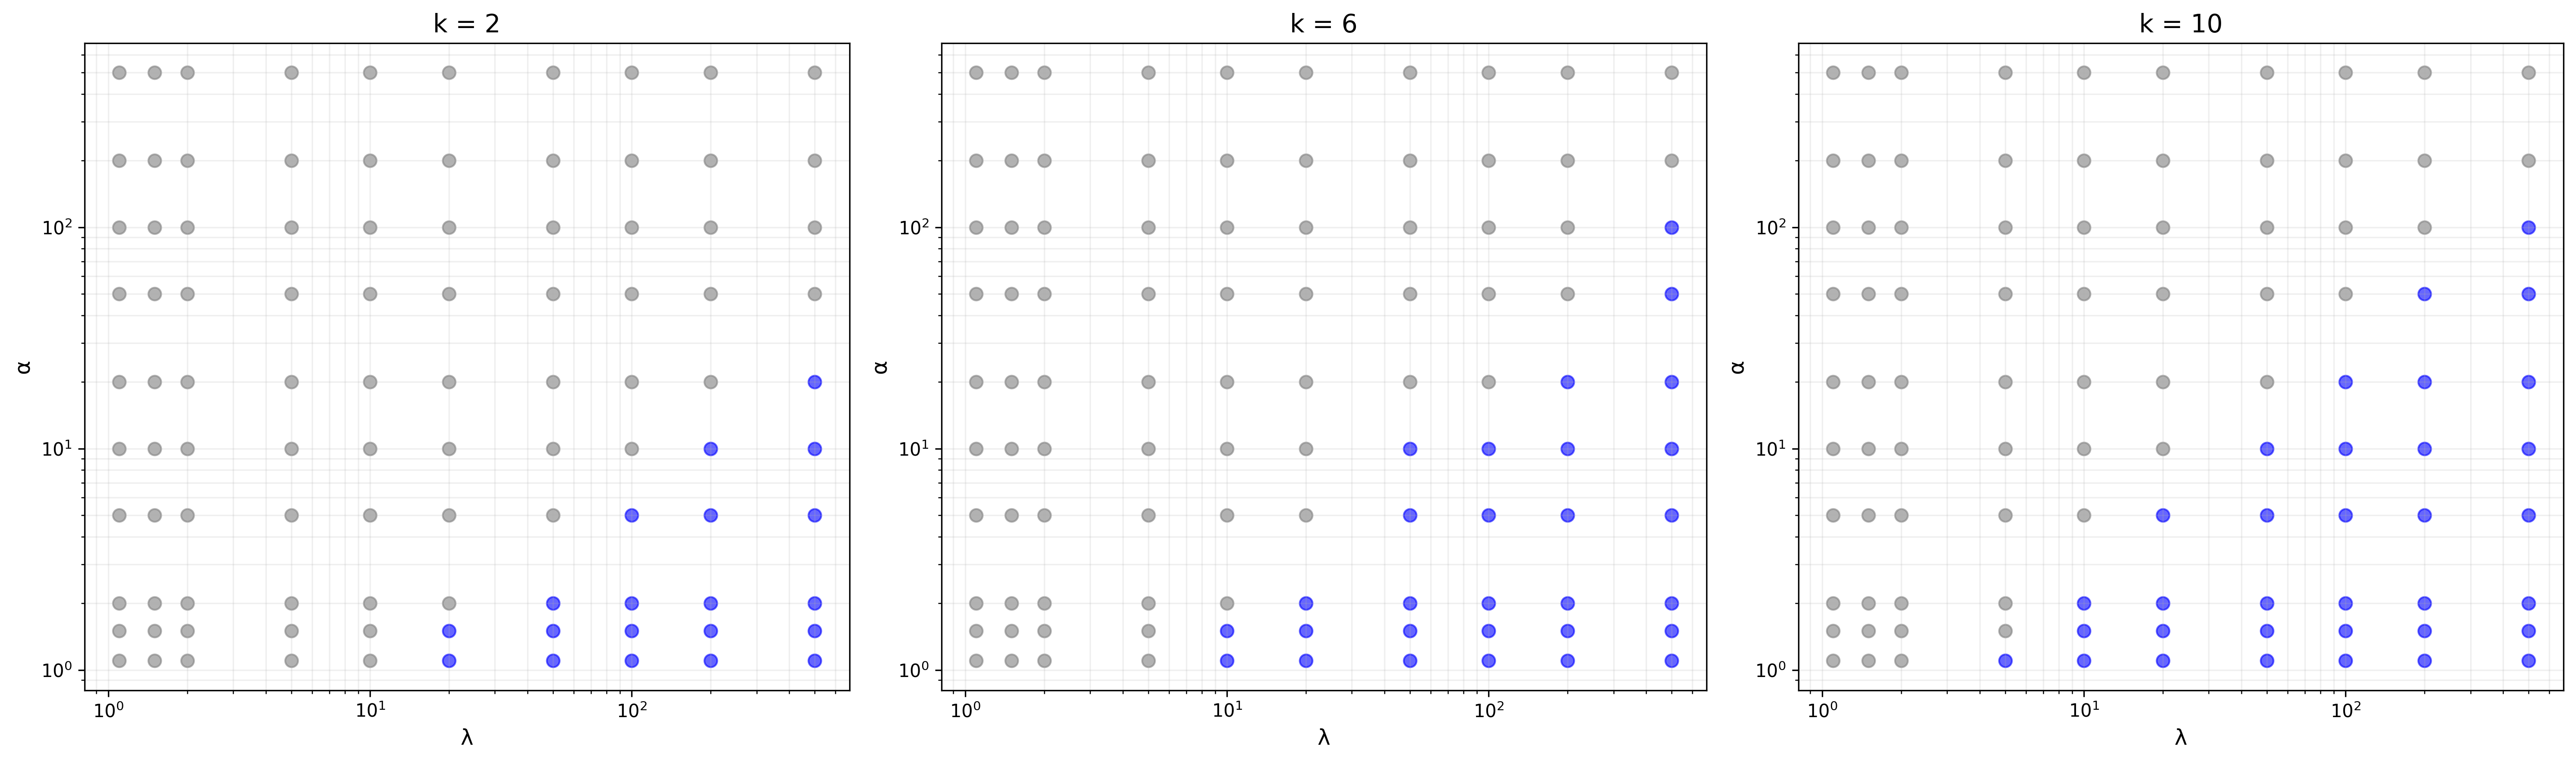
\includegraphics[width=0.95\textwidth]{figures/sleep-results.png}
    \caption{Results for our sleep simulations. Blue dots indicate when sleep is favored.}
    \label{fig:sleep-results}
\end{figure}

Figure 5 shows our simulation results for a variety of $k$, $\lambda$, and $\alpha$ and fixed $N = 100$. Blue dots indicate that the sleep was favored, while gray dots indicate that sleep was not favored. First, the logical conclusions that larger $\lambda$ would favor sleep more and larger $\alpha$ would favor awake more are true. Additionally, when $k$ is larger, the system is more likely to favor sleep. While have not yet produced an exact equation that models when sleep is beneficial (we would need to run larger simulations and do more sophisticated statistical analysis), the sleep appears to be favored when:
\begin{equation}
    \frac{\lambda}{\alpha} > F(k)
\end{equation}
where $F(k)$ is some function of $k$. This is very similar to the results found in Ohtsuki et al. (2006) with collaboration versus defection. We can conclude (under this simplified model) that even though sleep makes an individual more likely to die, the population can favor it when the benefit is significantly large. 

\section{Discussion and Future Work}
There are an endless number of biological and sociological scenarios that could be modeled by game theory on graphs and other related data structures. Our brief exploration into the implications of sleep provides one such direction. The simplified, binary model of sleep that we explored is certainly far from reality, and analyzing more complex patterns of sleep that include, for example, time series information or quality of sleep, can provide potential biological insights on why we (and most species) sleep. Additionally, the sleep simulations could be generalized onto other situations where there is some strategy that carries a risk of individual death but has large payouts for the population. 

Psychiatric conditions could also be considered as a beneficial target of analysis. Prior works in evolutionary dynamics generally assume that each node follows its strategy perfectly and that the games play out rationally. From a game-theoretic perspective, it is necessary that the games follow according to the rules; however, we can empirically see that humans in the real world do not always act rationally or follow perfectly the strategies that they believe to follow. Understanding how this irrational noise should actually be modeled can make the models map much more realistically onto reality. A concrete way to explore deviations from rational expectations is by examining how different psychiatric conditions could change the games. For example, if a node has social anxiety, it may be less likely to create connections with neighbors, and if a node has bipolar disorder, it may switch strategies in an extreme and unpredictable manner. Understanding the theoretical implications of psychiatric conditions in this way could have benefits for the field of computational psychiatry, which already is seeking to better understand psychiatric conditions from a generally data-first perspective. 

Considering psychiatry from a model-first perspective to merge it with the data-first community of computational psychiatry brings forth a broader point about research on evolutionary dynamics. The main downside of model-first approaches is that they can easily oversimplify or be disconnected to reality, meaning that their models can not accurately simulate actual elements of life. On the other hand, the main downside of data-first approaches is that data can be limited, flawed, biased, and the models that come out of the data can be over-fitted or simply incorrect for many cases outside of the dataset. However, there is no reason that these two perspectives cannot be bridged. Research could be done from a hybrid perspective, where model-first theoretical results are analyzed in order to guide studies conducted by the data-first approach, and the data from the data-first approach is used to guide theoretical models. This tight feedback loop would make both sides more grounded in reality and have more mathematical precision. Too often are the fields of pure mathematics and experimental sciences separated when there is undoubtedly benefits to having them tightly coupled. 


\section{Conclusion}
The combination of graph theory and evolutionary game theory provides a powerful framework for analyzing how strategies spread through populations. While the mathematical models we have discussed necessarily abstract away much of the complexity found in nature, they reveal fundamental principles about when cooperation, defection, and other strategies become dominant. Our extension of these models to incorporate sleep demonstrates how the framework can be expanded to study novel behavioral strategies. The simulations we conducted suggest that sleep is a natural strategy when it has sufficient benefit, even if it increases the chance of death for an individual. Though these theoretical results cannot fully capture the intricacies of biological and social evolution, they generate testable predictions and help guide empirical research. Future work should focus on bridging the gap between these abstract models and experimental studies, while continuing to explore how graph-theoretic approaches can theoretically explain evolutionary dynamics across different contexts.



\section{References}
\begin{hangparas}{0.5in}{1}

Allen, B., Lippner, G., Chen, Y. T., Fotouhi, B., Momeni, N., Yau, S.T., \& Nowak, M. A. (2017). Evolutionary dynamics on any population structure. Nature, 544, 227-230. \url{https://doi.org/10.1038/nature21723}

Fujimoto, Y., \& Ohtsuki, H. (2023). Evolutionary stability of cooperation in indirect reciprocity under noisy and private assessment. Proceedings of the National Academy of Sciences, 120(20), e2300544120. \url{https://doi.org/10.1073/pnas.2300544120}

Kobayashi, Y., Wakano, J. Y., \& Ohtsuki, H. (2015). A paradox of cumulative culture. Journal of Theoretical Biology, 379, 79-88. \url{https://doi.org/10.1016/j.jtbi.2015.05.002}

Lieberman, E., Hauert, C., \& Nowak, M. (2005). Evolutionary dynamics on graphs. Nature, 433, 312-316. \url{https://doi.org/10.1038/nature03204}

Ohtsuki, H., Hauert, C., Lieberman, E., \& Nowak, M. A. (2006). A simple rule for the evolution of cooperation on graphs and social networks. Nature, 441, 502-505. \url{https://doi.org/10.1038/nature04605}

Ohtsuki, H., Iwasa, Y., \& Nowak, M. A. (2015). Reputation effects in public and private interactions. PLOS Computational Biology, 11(11), e1004527. \url{https://doi.org/10.1371/journal.pcbi.1004527}

Walker, M. (2017). Why we sleep: The new science of sleep and dreams. Allen Lane (UK), Scribner (US).

\end{hangparas}

\end{document}
